\chapter{Definisi Kecerdasan Buatan}

\section{Apa itu kecerdasan buatan?}
\par Kecerdasan buatan terdiri dari dua kata yaitu "kecerdasan" dan "buatan", kecerdasan dasarnya adalah dari kata cerdas, cerdas adalah ketepatan dari sebuah pertanyaan yang diberikan atau sebuah ketepatan respon dari sebuah pernyataan yang diberikan yang selaras dengan kecepatan waktu tingkat kecerdasan akan semakin tinggi ketika tingkat ketepatan yang tinggi dan waktu yang rendah. Buatan dasarnya adalah dari kata buat, yang dimana hasil pekerjaan yang sudah dilakukan dimasa lampau. Kecerdasan buatan adalah sebuah program komputer yang dibuat agar mencapai keadaan dimana sebuah sistem bisa memberikan respon dengan tingkat ketepatan yang tinggi dan waktu yang rendah.

\section{Sejarah AI atau Kecerdasan Buatan}

\subsection{1943 - 1950}
\par Awalnya AI dikerjakan oleh dua orang yaitu Warren McCulloch dan Walter Pits pada tahun 1943. Mereka membangun sebuah AI dengan berlandaskan 3 poin, yaitu:
\begin{enumerate}
    \item Pengetahuan dasar tentang psikologi dan fungsi saraf neuron pada otak manusia.
    \item Logika analisis berdasarkan prinsipal matematika Russell dan Whitehead.
    \item Teori komputasi turing.
\end{enumerate}
\par Mereka menghasilkan sebuah model kecerdasan buatan dari konsep jaringan saraf dan membuktikan bahwa komputer bisa belajar. Pada tahun 1950 dua mahasiswa Harvard membuat sebuah komputer untuk memproses kerja jaringan saraf yang membutuhkan 3000 tabung vakum untuk menjalankan 40 neurons.

\subsection{1980 - sekarang}
\par Kecerdasan buatan sudah mencapai tahap industri dimana beberapa aspek sudah menggunakan kecerdasan buatan dalam penerapan dilapangan, contohnya adalah pada industry perbankan sebuah komputer bisa membaca tulisan tangan dari manusia sehingga bisa mempercepat proses pengisian administrasi.

\subsection{1986 - sekarang}
\par Penggunaan algoritma neural networks (jaringan saraf) dikarenakan pada pertengahan tahun 1980 - 1990 adanya suatu masalah yang dimana sebuah algoritma sudah melakukan kesalahan dalam pembelajaran pada komputer.

\subsection{2001 - sekarang}
\par Dataset yang sangat melimpah dan diikuti dengan algoritma kecerdasan buatan yang semakin baik dalam pembuatan model dengan akurasi yang tinggi, membuat banyak cabang AI contohnya seperti mobil yang bisa menyetir sendiri dengan bantuan komputasi, pengenalan suara, pengenalan teks, sebuah komputer yang layaknya manusia jika diajak pesan daring, robotik, dan banyak lainnya.

\section{supervised learning}
\par supervised learning adalah metode pembelajaran sebuah komputer dengan cara pengklasifikasian sebuah sample data training yang memiliki label setiap samplenya, kita asumsikan bahwa A penyuka sepakbola dan A sudah hafal semua logo tim sepakbola didunia dengan hanya melihat logo tim sepakbola A bisa mengetahui dari liga mana tim sepakbola itu berasal, cara A belajar adalah dengan memberikan label pada setiap tim sepakbola yang dia lihat bahwa tim ini berasal dari liga inggris, tim itu berasal dari liga italia, sehingga metode pembelajarannya memberikan klasifikasi pada setiap tim sepakbola yang ada.

\section{klasifikasi}
\par pengelompokkan sebuah data sampel berdasarkan label yang sudah ada pada data sampel yang bertujuan untuk pembelajaran komputer untuk bisa merespon pertanyaan atau pernyataan yang diberikan tanpa ada label pada pertanyaan ataupun pernyataan yang diberikan.

\section{regresi}
\par regresi akan menghasilkan sebuah variabel yang bisa digunakan kembali untuk pernyataan ataupun pertanyaan selanjutnya, contohnya: berapa panjang kaki seseorang berdasarkan usia, berat badan, dan tinggi badan seseorang.

\section{unsupervised learning}
\par perbedaan unsupervised learning dengan supervised learning adalah ketika SL menggunakan klasifikasi sedangkan UL menggunakan clustering, kita asumsikan A sedang belajar tim-tim sepakbola dari liga mana saja. Maka dari data sampel yang dimiliki A dia tidak menemukan dari liga mana saja tim sepakbola berasal, maka dari itu A melakukan clustering dimana mengelompokan tim mana saja yang berada dikota negara itali, tim mana saja yang berada dikota negara inggris, sehingga nantinya A akan mengetahui tim sepakbola berasal dari liga mana saja.

\section{Installasi library scikit-learn}
\par Perintah yang diketikkan pada shell/cmd adalah \textbf{pip install scikit-learn}.
\begin{figure} [H]
    \centering
    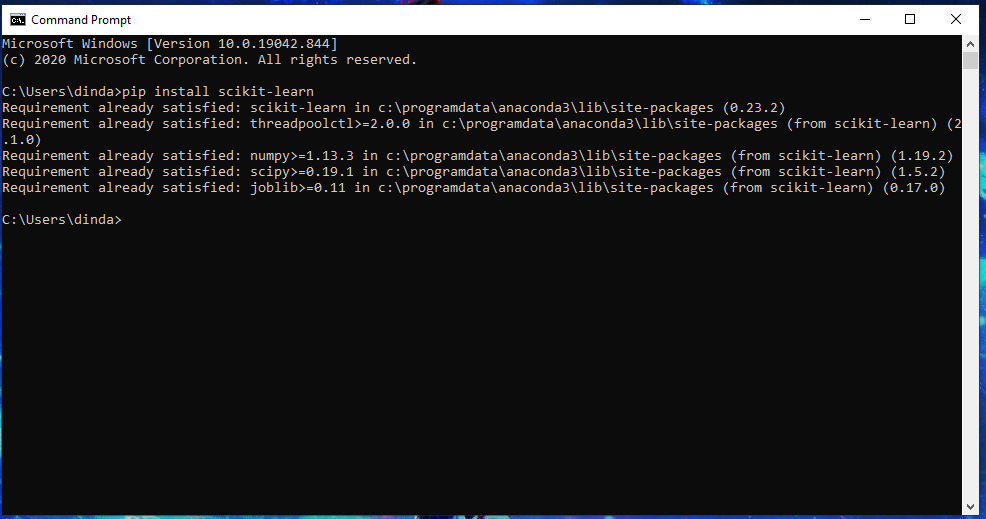
\includegraphics[scale=0.6]{figures/install_scikit_learn.PNG}
    \caption{Installasi scikit-learn}
    \label{fig:install_scikit_learn}
\end{figure}

\begin{enumerate}

\item
Mencoba Loading an example dataset, menjelaskan maksud dari tulisan tersebut dan mengartikan per baris.\\

Loading an example dataset (memuat contoh kumpulan data) maksudnya yaitu scikit-learn memugkinkan kita untuk mengambil atau memuat data standar, misalnya kita mengambil atau memuat data set iris dan digits untuk membuat sebuah klasifikasi dan data set diabetes untuk regresi.\\

\begin{lstlisting}[language=Python]
def loadingAnExample():
    iris = datasets.load_iris()
    digits = datasets.load_digits()
    print(digits.images[0])
\end{lstlisting}

\item
Mencoba Learning and predicting, menjelaskan maksud dari tulisan tersebut dan mengartikan per baris.\\

Learning and Predicting (Belajar dan Memprediksi) maksudnya yaitu belajar dari sebuah model dan membuatkan prediksi dalam sebuah gambar. Menggunakan data set digits karena data digits dapat memprediksi, mengingat gambar digit mana yang diwakilinya. \\

\begin{lstlisting}[language=Python]
def learningAndPredicting():
    digits = datasets.load_digits()
    clf = svm.SVC(gamma=0.001, C=100.) #parameter model

    data = clf.fit(digits.data[:-1], digits.target[:-1]) #fit x, y
    print(data)

    prediksi = clf.predict(digits.data[-1:]) #predict T (hasil prediksi data baru)
    print(prediksi)
\end{lstlisting}

\item
mencoba Model persistence, menjelaskan maksud dari tulisan tersebut dan mengartikan per baris.\\
Model Presistence maksudnya mempertahankan sebuah model agar bisa digunakan di masa depan tanpa perlu melatih kembali atau membuat model itu kembali. Menyimpan model dengan menggunakan pickle atau joblib

\begin{lstlisting}[language=Python]
def modelPresistence():
    clf = svm.SVC()
    X, y = datasets.load_iris(return_X_y=True)
    print(clf.fit(X, y))

    #contoh menggunakan pickle
    s = pickle.dumps(clf)
    clf2 = pickle.loads(s)
    print(clf2.predict(X[0:1]))

    print(y[0])

    #contoh menggunakan joblib
    to_persist = [('a', [1, 2, 3]), ('b', np.arange(10))]
    dump(to_persist, 'filename.joblib')

    # dump(clf, 'filename.joblib')
    # clf = load('filename.joblib')

    print(load('filename.joblib'))
\end{lstlisting}

\item 
Mencoba Conventions, menjelaskan maksud dari tulisan tersebut dan mengartikan per baris.\\

Conventions (konvensi) maksudnya dapat memprediksi dengan lebih prediktif.\\

\begin{lstlisting}[language=Python]
def conventions():
    #type casting
    rng = np.random.RandomState(0)
    X = rng.rand(10, 2000)
    X = np.array(X, dtype='float32')
    print(X.dtype) #type float 32

    transformer = random_projection.GaussianRandomProjection()
    X_new = transformer.fit_transform(X)
    print(X_new.dtype) #type float 64

    # jika type tidak ditentukan, maka akan diformat langsung ke type float 64
    iris = datasets.load_iris()
    clf = SVC()
    print(clf.fit(iris.data, iris.target))

    print(list(clf.predict(iris.data[:3])))

    print(clf.fit(iris.data, iris.target_names[iris.target]))

    print(list(clf.predict(iris.data[:3])))

    #Refitting and updating parameters
    #memperbaiki dan memperbarui parameter
    X, y = load_iris(return_X_y=True)

    print(clf.set_params(kernel='linear').fit(X, y))
    print(clf.predict(X[:5]))

    print(clf.set_params(kernel='rbf').fit(X, y))
    print(clf.predict(X[:5]))

    #Multiclass vs. multilabel fitting
    X = [[1, 2], [2, 4], [4, 5], [3, 2], [3, 1]]
    y = [0, 0, 1, 1, 2]

    classif = OneVsRestClassifier(estimator=SVC(random_state=0))
    print(classif.fit(X, y).predict(X)) #klasifikasi array 1 dimensi

    # klasifikasi array 2 dimensi yang mewakili prediksi multilabel
    y = LabelBinarizer().fit_transform(y)
    print(classif.fit(X, y).predict(X))

    # klasifikasi array 2 dimensi dengan beberapa label yang diprediksi untuk setiap instans.
    y = [[0, 1], [0, 2], [1, 3], [0, 2, 3], [2, 4]]
    y = MultiLabelBinarizer().fit_transform(y)
    print(classif.fit(X, y).predict(X))
\end{lstlisting}

\end{enumerate}